\documentclass[11pt,a4paper]{article}

\usepackage[T1]{fontenc}
\usepackage[utf8]{inputenc}
\usepackage[frenchb]{babel}

\usepackage{fancyhdr} % headers
\usepackage[usenames,dvipsnames]{color} % colors
\usepackage{graphicx} % images
\usepackage{listings} % source code
\usepackage{titling} % meta-infos
\usepackage{courier} % courier font
\usepackage{fullpage} % full page layout
\usepackage{titlesec} % title customization
\usepackage{parskip} % paragraphs spacing
\usepackage{amsmath}
\usepackage{tikz}
\usepackage{siunitx}
\usepackage{tabularx}
%\usepackage{showframe} % layout debug

\usepackage{float}
\restylefloat{figure}
\usepackage[nottoc,numbib]{tocbibind}

\topmargin -10mm
\headsep 8mm
\headheight 10mm

\linespread{1.0}
\renewcommand{\arraystretch}{1.3}

\setlength{\unitlength}{1cm}
\setlength{\droptitle}{5cm}

\pagestyle{fancy}
\fancyhf{}
\cfoot{\thepage}

\def \doccourse { INF2-B -- Présentation }
\def \doctitle {Gestion de versions avec Git}
\author{Bastien Clément \and Christophe Peretti}

\rhead{\theauthor \\ \today}
\lhead{\doccourse \\ \doctitle }
\title{{\normalsize \doccourse} \\ \doctitle }

\begin{document}
\pagenumbering{gobble}

\maketitle

\vspace{3cm}
\begin{center}

\includegraphics[width=5cm]{git_logo}
\end{center}

\pagebreak
\pagenumbering{roman}

\tableofcontents

\pagebreak
\pagenumbering{arabic}

\section{Introduction à la gestion de versions}

\textit{Git} est un logiciel de gestion de versions libre et open-source.
Avant de s'y attaquer directement, il est nécessaire de commencer par une petite introduction sur le concept de gestion de version.
De quoi s'agit-il et pourquoi est-ce intéressant dans le domaine de la programmation logiciel ?

Basiquement, un logiciel de gestion de versions se charge d'enregistrer les modifications apportées à un ensemble de fichier au cours du temps.
Par la suite, il permet de naviguer dans cet historique pour consulter ou récupérer d'anciennes versions d'un fichier particulier.
Dans notre cas, nous l'utiliserons typiquement pour conserver l'historique du code source de nos programmes.

\subsection{Gestion de versions locale}

Une façon de mettre en place un simple de gestion de versions très basique serait d'effectuer périodiquement des copies du projet en les annotant avec la date et l'heure.
Il serait alors possible de retourner dans une copie particulière pour avoir accès à une version antérieur d'un fichier.

Des logiciels automatiques sur le même principe sont même intégrés directement aux système d'exploitation comme par exemple \textit{Time Machine} sur OS X et \textit{File History} sur Windows.
Ces sauvegardes sont cependant effectuées automatiquement à intervalles fixes et ne correspondent pas aux étapes du développement du logiciel.

\iffalse %%%
\begin{figure}[h]
\begin{center}
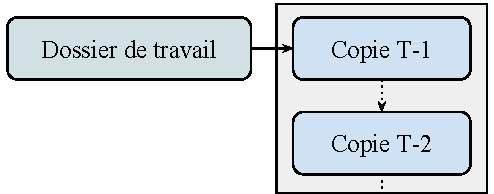
\includegraphics[width=7.2cm]{img_lvcs} \\
\caption{Exemple de gestion de versions locale simple}
\end{center}
\end{figure}
\fi %%%

Les logiciels spécialisés (tel que \textit{rcs}, développé depuis 1982) permettent à l'inverse d'effectuer des sauvegardes à des moments particuliers, typiquement lorsqu'une fonctionnalité du programme est terminée et prête à être enregistrée.
Ces logiciels fournissent ainsi un niveau de \textit{sécurité} et d'\textit{historique}, constituant les premières facettes de la gestion de versions.

\subsection{Gestion de versions centralisée}

%Une autre facette de la gestion de versions est la \textit{collaboration}. 

Le développement de logiciels, pour tout projet un minimum sérieux, implique généralement la collaboration de plusieurs développeurs.
Même dans le cadre de nos laboratoires encore relativement simples, nous avons pu constater les difficultés liées au développement à plusieurs.
Comment rester à jour sur le travail effectué par notre binôme ?
Comment garder une copie cohérente du projet lorsqu'un fichier est modifiés par plus d'une personne au même moment ?

Les logiciels de gestion de versions centralisés règlent ce problème en se basant sur un \textit{dépôt} central dans lequel les fichiers constituant la version de référence du logiciel sont enregistrés.
C'est le cas par exemple du logiciel \textit{Subversion} (souvent abrégé \textit{svn}).

\iffalse
\begin{figure}[ht]
\begin{center}
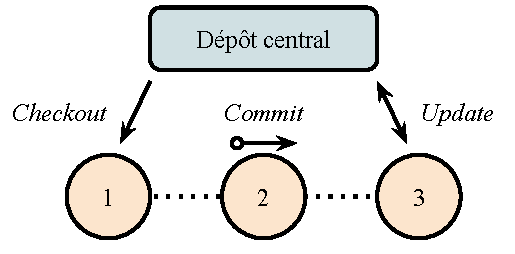
\includegraphics[width=8cm]{img_cvcs}
\caption{\textit{Workflow} typique d'un système de gestion de versions centralisé}
\end{center}
\end{figure}
\fi

Lorsqu'un développeur souhaite modifier le logiciel, il commence par en effectuer une copie sur sa machine (opération \textit{checkout}), modifie et enregistre son travail localement (opération \textit{commit}), puis il termine en envoyant ses modifications sur le dépôt central (opération \textit{update}) pour qu'elles soient intégrées définitivement au logiciel.
Il récupère au passage les modifications des autres développeurs et est informés des situations de conflits, c'est à dire deux modifications différentes sur la même partie de code, qu'il doit résoudre avant de pouvoir continuer.

Dans cette configuration, le dépôt central constitue un \textit{single point of failure}.
S'il est inaccessible, la collaboration et l'envoi des modifications deviennent temporairement impossible.
Si un problème plus grave survient, en l'absence de sauvegarde récente, une partie ou l'ensemble de l'historique du projet peut être définitivement perdu ou corrompu.

\subsection{Gestion de versions distribuée}

À l'inverse, dans un système décentralisé tel que Git (mais aussi \textit{Mercurial} ou \textit{Bazaar}), lorsqu'une copie locale du projet est effectuée, ce n'est pas uniquement les dernières versions des fichiers qui sont récupérées, mais l'ensemble de l'historique du dépôt.
On parle alors de \textit{clônage}.

Il n'y a ainsi plus de dépôt central à proprement parler et chaque développeur possède naturellement un copie complète de l'historique du projet.
La majorités des opérations peuvent ainsi s'exécuter hors-ligne avec d'excellentes performances.

L'absence de dépôt central permet également d'organiser le développement de façon très flexible selon ce qui est le plus adapté à chaque situation.
En utilisant un unique dépôt en ligne et accessible de tous, Git peut même reproduire l'organisation typique d'un système centralisé.

\begin{figure}[ht]
\begin{center}
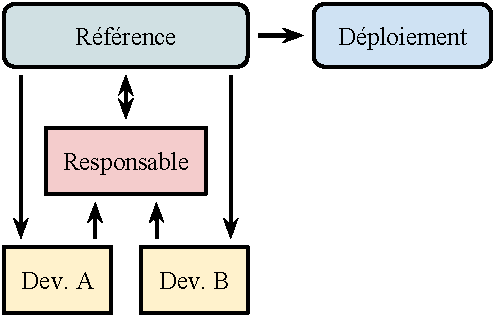
\includegraphics[width=11.5cm]{img_dvcs}
\caption{Exemple d'organisation décentralisée avec un \textit{responsable d'intégration}}
\end{center}
\end{figure}

Dans l'exemple donné, les développeurs clônent le dépôt de référence et effectue leurs modifications localement.
Ils les publient ensuite dans un dépôt publiquement accessible et demande au responsable de récupérer les changements pour les intégrer dans le dépôt officiel après validation.

%C'est le modèle encouragé par la plateforme GitHub (que nous aborderons plus tard) puisqu'il favorise une collaboration spontanée aux projets.
%Il n'y a besoin d'aucun accord ou droit d'accès particulier pour pouvoir commencer à modifier le logiciel original.
%Le responsable du projet n'est impliqué qu'une fois la modification terminée et en principe testée. Il ne lui reste plus qu'à relire les changements et décider de l'intégrer ou non au projet officiel.

\section{Git}

%Cette seconde partie abordera des points plus spécifique à Git: les origines du projet, ses principales caractéristiques mais aussi quelques points sur l'organisation interne du dépôt.

\subsection{Histoire}

L'histoire du projet Git est étroitement liée au développement du noyau Linux, développés tous deux par Linus Torvalds.

Dans un premier temps, de 1991 à 2002, les développeurs et contributeurs de Linux n'utilisaient pas de logiciels particuliers et échangeaient leur travail sous forme de \textit{patches} et d'archives.
Face aux difficultés engendrées par la croissance du projet, la décision d'utiliser le logiciel de gestion de versions propriétaire BitKeeper est prise.
L'éditeur proposait alors une licence gratuite permettant, sous certaines conditions, d'utiliser gratuitement une version limitée de son logiciel pour le développement de logiciels libre.

En 2005, un conflit entre un développeur indépendant de l'organisation OSDL (\textit{Open Source Development Labs}) et la société éditrice BitMover conduit à la résiliation de la licence particulière pour les logiciels libres.
Bien que BitMover propose de continuer à fournir gratuitement son logiciel à certains développeurs de Linux, elle le refuse à Linus Torvalds, également membre de l'OSDL.
L'utilisation de BitKeeper est alors abandonnée et le projet Git est lancé avec pour but de devenir le nouveau logiciel de gestion de versions utilisé par les développeurs du noyau Linux.

\subsection{Caractéristiques}

Destiné à l'un des plus grand projet open-source existant, Git a été conçu dès le départ avec beaucoup d'exigences sur la base de ce qui avait été appris avec l'utilisation de BitKeeper.

\begin{enumerate}
	\item {Entièrement distribué}, 
	il n'y a aucun dépôt fondamentalement plus important.
	
	\item {Gestion du développement non-linéaire},
	même avec des milliers de branches simultanées.
	
	\item {Capable de support de très gros projets}
	tel que Linux tout en conservant vitesse d'exécution et optimisation de l'espace disque.
\end{enumerate}

Au fil du temps, Git a évolué en conservant ces caractéristiques faisant de lui un excellent logiciel dans son domaine.
Il est maintenant largement utilisé en dehors du développement de Linux.

\subsection{Chaîne de révisions}

Le fonctionnement de Git peut être comparé à celui d'un système de fichiers (tel que celui qui gère les fichiers d'un disque dur) sur lequel on a greffé des fonctionnalités de gestions de versions.
En effet, un dépôt n'est rien d'autre qu'une structure de répertoire et de fichiers associé à leur contenu.

Lorsque l'utilisateur enregistre une nouvelle version de son projet (appelée \textit{commit} ou \textit{révision}), un \textit{snapshot} de l'état actuel des fichiers est enregistré dans l'historique du dépôt.
Par optimisation, lorsqu'un fichier n'a pas été modifié, le contenu du snapshot précédent est réutilisé tel quel. Les dernières versions des fichier sur lesquels travail l'utilisateur (le \textit{répertoire de travail}) sont à la fin de la chaine et formeront la prochaine révision du projet lors du commit.

\begin{figure}[ht]
\begin{center}
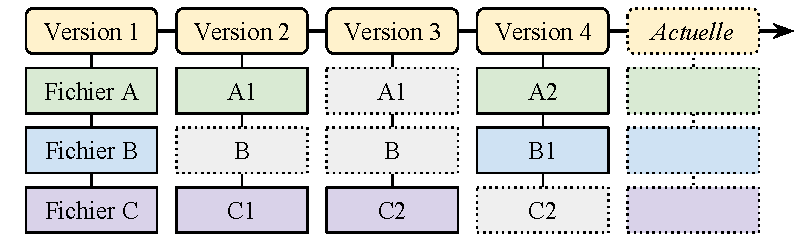
\includegraphics[width=12cm]{img_snapshots}
\caption{L'historique du dépôt est une séquence de snapshots des fichiers du projet}
\end{center}
\end{figure}

\subsection{\textit{Staging area}}

En réalité, le répertoire de travail ne forme pas directement la prochaine révision du projet.
Git possède en effet la particularité d'utiliser un espace intermédiaire appelé \textit{staging area} dans lequel sont manuellement placés les fichiers à sauvegarder lors du prochain commit. 

Ceci permet de sélectionner avec précision quels fichiers, voir quelles lignes de ceux-ci, devront être capturés et ainsi ignorer certaines modifications dont la sauvegarde ne serait pas pertinente au commit actuel et devraient faire l'objet d'une révision séparée.

L'utilisation de nombreux petits commit permet d'obtenir un historique plus précis et facilite certaines opérations comme par exemple l'annulation (\textit{revert}) d'un changement spécifique. Si plusieurs changements indépendants sont rassemblés en un commit, l'historique perd en clarté.

%Par exemple, deux modifications complètement indépendantes pourront par la suite plus facilement être annulées si elle sont enregistrée séparément dans l'historique.

\begin{figure}[ht]
\begin{center}
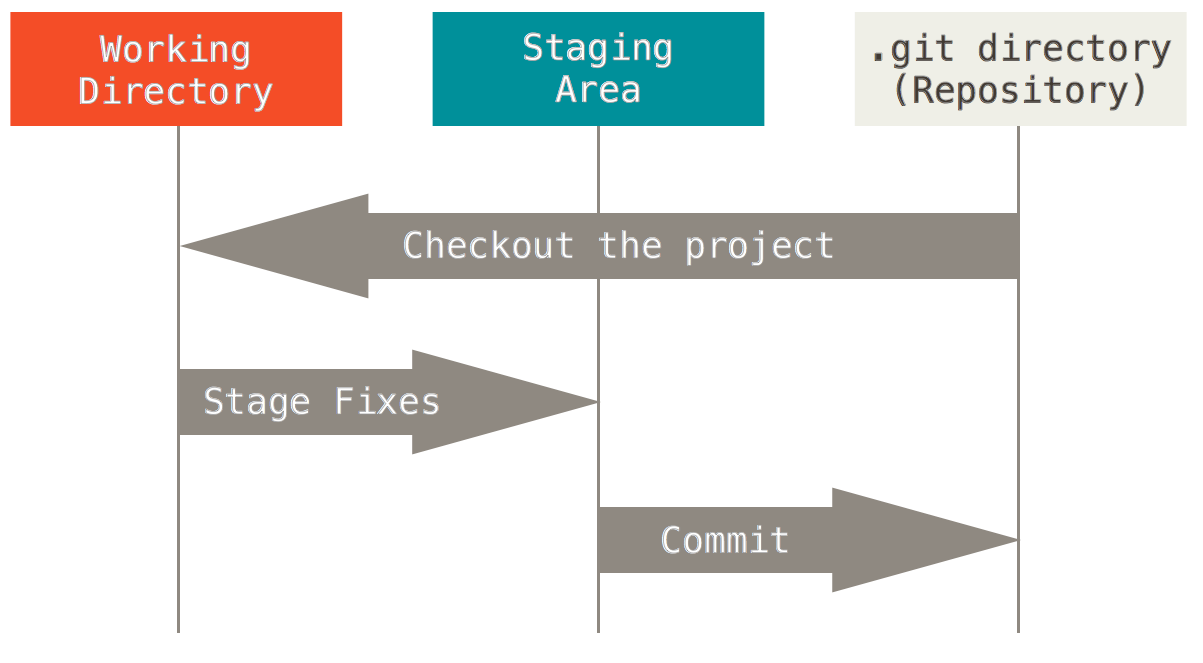
\includegraphics[width=9cm]{img_areas} \cite{progit}
\caption{Les trois zones dans lesquels résident les fichiers gérés par Git}
\end{center}
\end{figure}

\vspace{-4mm}
\subsection{Stockage adressé par contenu}

La base de donnée de Git est un \textit{stockage adressé par contenu} (en anglais \textit{Content Addressable Storage}, c'est à dire une base de données qui identifie les informations sur la base de leur contenu plutôt que d'une clé ou d'un nom.
Il est donc nécessaire de connaître le contenu de ce que l'on souhaite récupérer ce qui peut sembler paradoxal.

Le système se base sur la fonction de hachage cryptographique SHA-1.
Tout ce qui est contenu dans l'historique est premièrement hashé puis enregistré sur le disque à un emplacement qui dépend de la valeur obtenue.
Pour retrouver cette information, il est indispensable d'enregistrer ce hash quelque part, constituant ainsi un \textit{pointeur} contenant l'\textit{adresse} d'une information.

Il y a principalement trois types d'objet dans la base de donnée de Git:

\begin{enumerate}
	\item Les {\bf commits},
	ils contiennent l'ensemble des méta-informations d'une révision particulière tel que l'auteur, la date et l'heure mais aussi l'adresse d'un tree représentant le dossier principal du projet et l'adresse du commit qui le précède, formant ainsi l'historique.
	
	\item Les {\bf trees},
	ils listent l'ensemble des fichiers et sous-dossier d'un répertoire particulier ainsi que l'adresse de leur contenu.
	L'adresse d'un sous-dossier sera l'adresse d'un autre \textit{tree}.
	
	\item Les {\bf blobs},
	ils sont les fichiers eux-mêmes.
\end{enumerate}

\begin{figure}[H]
\begin{center}
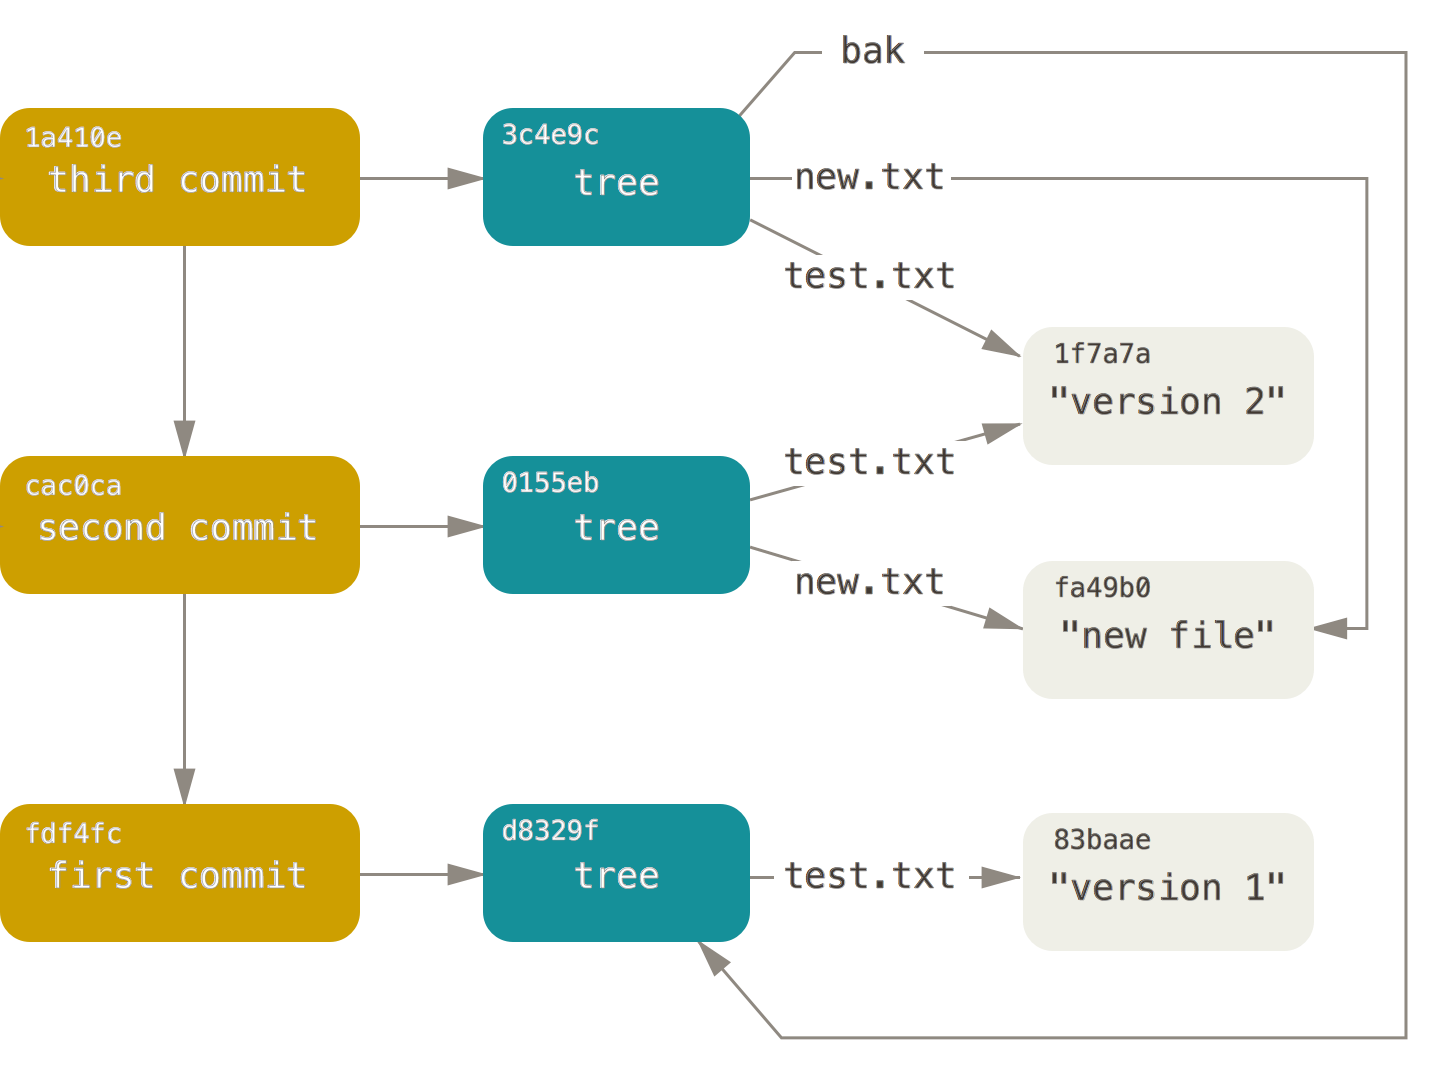
\includegraphics[width=9.1cm]{img_structure} \cite{progit}
\caption{Structure interne d'un dépôt Git avec \textit{commits}, \textit{trees} et \textit{blobs}}
\end{center}
\end{figure}

Puisque l'adresse d'un blob dépend de son contenu, il est évident qu'une modification entrainera un changement de l'adresse du \textit{blob} et que la propagation de ce changement dans les \textit{trees} entrainera un nouvel arbre raçine à une adresse différente, correspondant à une nouvelle révision.

Cette structure entraine naturellement deux propriétés très appréciables:

\begin{enumerate}
	\item \textbf{Déduplication}, 
	si une information est identique à une autre déjà contenue dans la base de données, leurs adresses seront identiques et le contenu existant sera simplement réutilisé.
	
	\item \textbf{Intégrité},
	l'adresse d'une information étant directement liée à son contenu, il est impossible qu'une corruption du dépôt ne passe inaperçue.
	Chaque bit d'information récupéré de la base de données est toujours identique à celui qui y a été enregistré.
\end{enumerate}

\section{Branches}

Jusqu'à maintenant, nous n'avons utilisé Git que pour enregistrer une séquence linéaire de modifications. Sa vraie force réside dans son excellent support de \textit{branches} représentant des modifications parallèles et indépendantes des fichiers du projet.

\iffalse
\begin{figure}[h]
\begin{center}
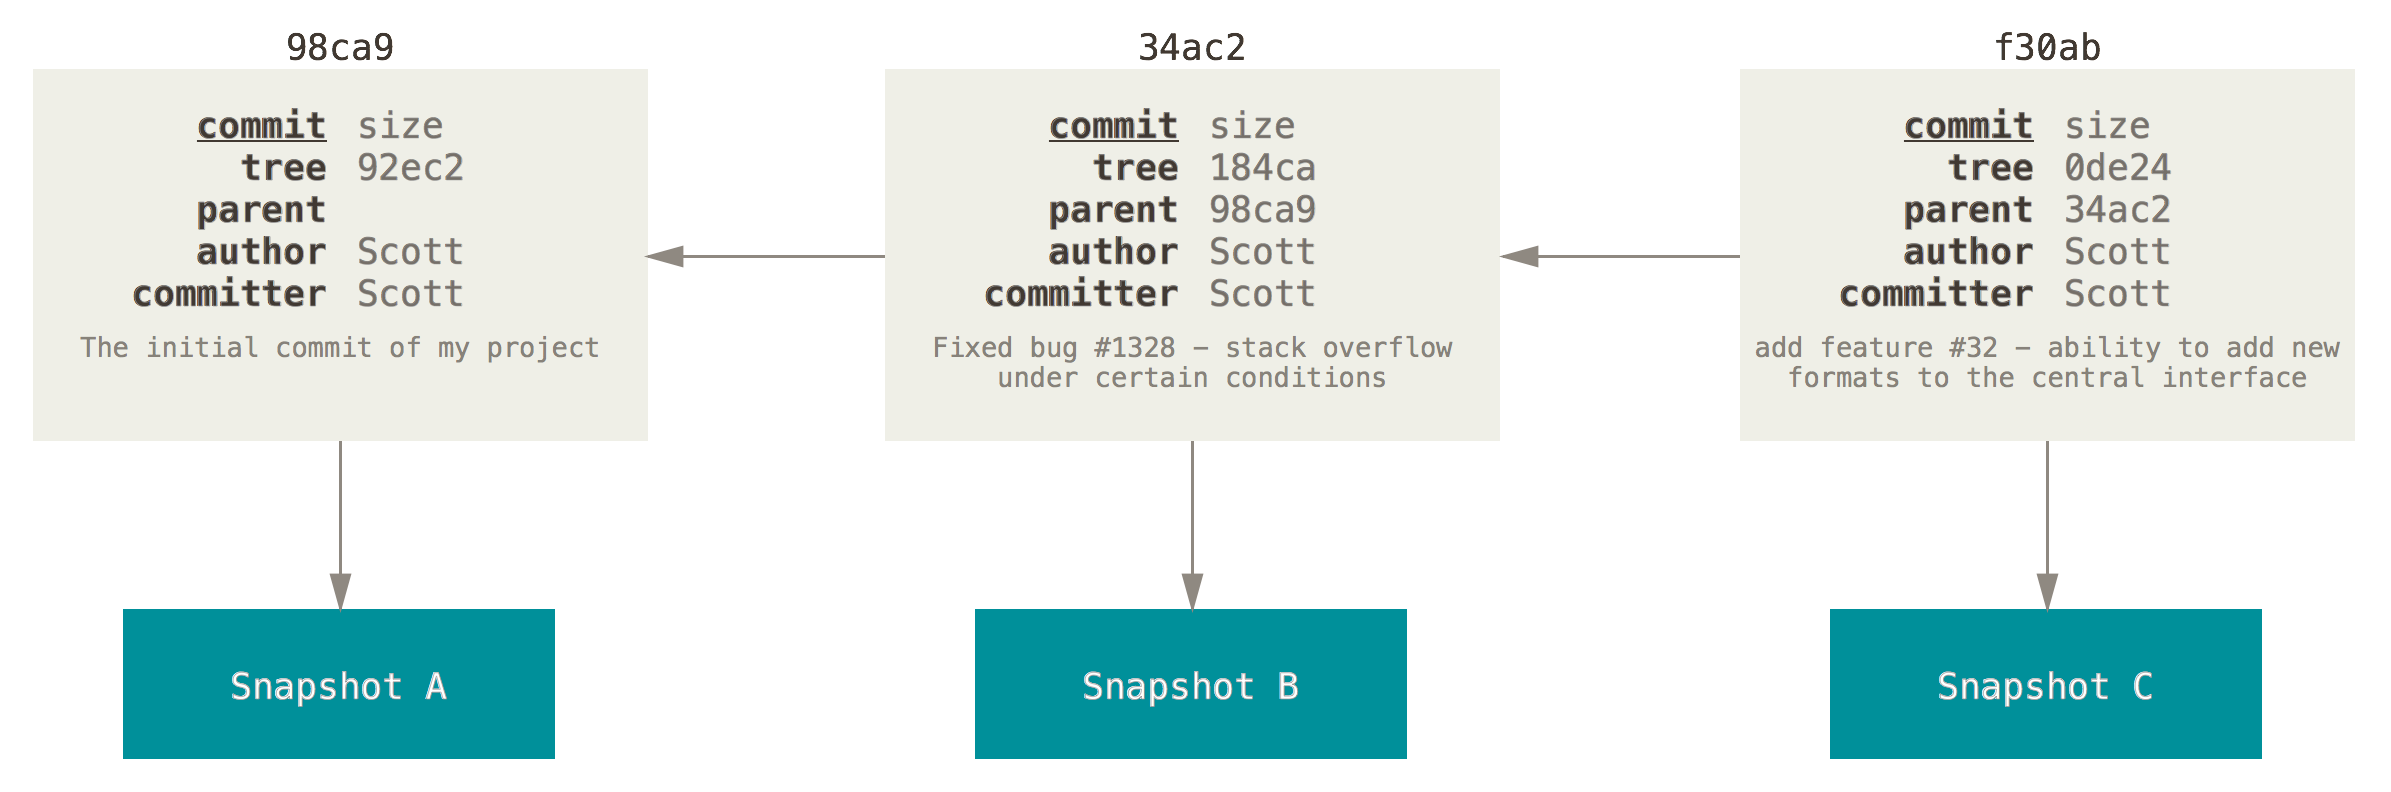
\includegraphics[width=11.5cm]{img_commits_chain}
\caption{Séquence linéaire de commits dans un dépôt}
\end{center}
\end{figure}
\fi

\subsection{Références}

Nous avons vu dans la section précédente comment l'historique du dépôt était organisé en interne. Il reste un dernier problème: comment obtenir l'adresse du dernier commit permettant ensuite d'accéder à l'ensemble de la structure ?

Cette information essentielle, appelée \textit{référence}, est enregistrée en dehors de la base de données principale et associe un nom à un commit spécifique. Chaque branche de développement correspond donc simplement à une référence particulière indiquant le dernier commit de cette branche. Par défaut, un dépôt Git ne contient qu'une seule branche appelée \textit{master}. Il est également possible pour plusieurs références de pointer vers le même commit.

\begin{figure}[h]
\begin{center}
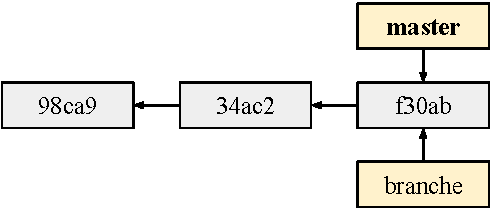
\includegraphics[width=6cm]{img_refs}
\caption{Deux références pointant vers le même commit}
\end{center}
\end{figure}

%Lors de l'enregistrement d'une nouvelle révision, la référence de la branche courante est avancée et pointe à présent sur le dernier commit de la chaîne.

\begin{figure}[h]
\begin{center}
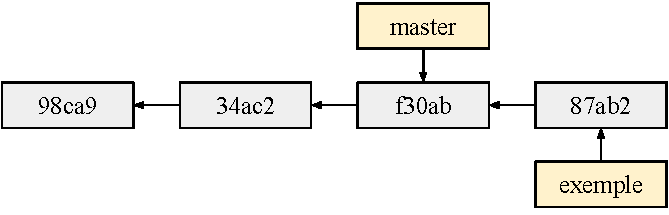
\includegraphics[width=8cm]{img_refs2}
\caption{Lors d'un commit, la référence de la branche courante est avancée}
\end{center}
\end{figure}

Il est à tout moment possible de changer la branche sur laquelle on travail. Les fichiers du répertoire de travail sont alors mis à jour pour refléter l'état dans lequel ils étaient lors du dernier commit de la branche en question.

\subsection{Divergences}

Que ce passe-t-il à présent si des modifications sont enregistrées sur la branche \textit{master} ? Nous sommes alors face à une situation de divergence où le développement du projet s'est divisé en deux branches distinctes et indépendantes.

\begin{figure}[h]
\begin{center}
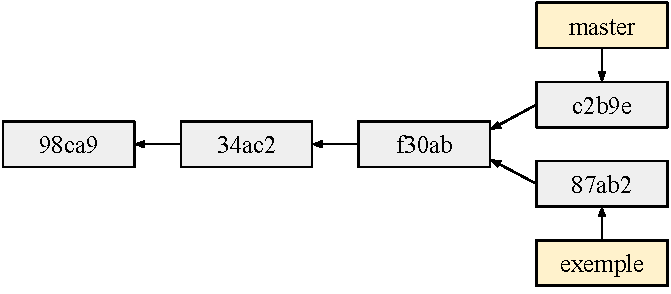
\includegraphics[width=8cm]{img_divergence}
\caption{Les branches \textit{master} et \textit{exemple} ont divergé}
\end{center}
\end{figure}

Il est par exemple possible d'utiliser ce mécanisme pour développer deux fonctionnalités indépendantes sans que le développement de l'une d'elles n'impacte le développement de l'autre.
C'est aussi implicitement la situation qui survient lorsque deux développeurs travaillent en parallèle sur la même version du logiciel, dans ce cas, il s'agit d'une divergence entre une branche et elle-même, mais dans un dépôt différent.

\subsection{Fusion}

Lorsque deux branches divergentes doivent être rassemblées en une seule, il est question de \textit{fusion} des branches.

\subsubsection{\textit{Fast-forward}}

\subsubsection{\textit{Rebasing}}

\subsubsection{\textit{Three-way merge}}

\subsection{Conflits}

\subsection{Tags}

\section{Conclusion}

Cette présentation aura permis de découvrir une vue d'ensemble du logiciel de gestion de versions Git ainsi que des exemples d'organisation et d'utilisation illustrant sa grande flexibilité. On remarque rapidement que l'utilisation d'un tel logiciel devient indispensable lors d'un développement logiciel, plus particulièrement dans le cas d'une collaboration de plusieurs développeurs.

\pagebreak
\pagenumbering{alph}
\section{Compléments}

\subsection{Téléchargement et installation de Git}

Git peut être téléchargé depuis le site officiel du projet {\tt http://git-scm.com/}.
Le logiciel est disponible pour tous les systèmes d'exploitation courants.

\subsection{GitHub}

Il est difficile aujourd'hui de présenter Git sans mentionner rapidement le site internet GitHub.

Lancé le 10 avril 2008, c'est un service indépendant d'hébergement et de gestion de développement de logiciels basé sur Git qui compte aujourd'hui plus de 9 millions d'utilisateurs.

GitHub fait partie des facteurs ayant contribué à l'adoption rapide de Git dans le monde de l'\textit{open source} et est aujourd'hui une plateforme incontournable utilisée de façon intensive par de grands noms tel que Google, Microsoft et Facebook. 

Destinée avant tout aux développeurs, l'interface est très simple et épurée, mettant l'accent sur le code source en tant qu'élément central du développement. Par exemple, la page principale d'un dépôt est simplement le navigateurs de fichier de ce dépôt suivi d'un fichier texte de description.

\subsection{Offre GitHub pour les étudiants}

L'hébergement de dépôt sur GitHub est entièrement gratuit pour les projets open-source.
En revanche, il est nécessaire souscrire à un abonnement pour pouvoir créer des dépôts privés dont l'accès est limité aux personnes autorisées.

Heureusement, les personnes possédant une adresse e-mail provenant d'une université reconnue (dont la HEIG-VD fait partie!) peuvent demander un plan \textit{Micro} gratuit pendant toute la durée des études, soit 5 dépôts privés avec un nombre illimités de collaborateurs par dépôt.

L'inscription se fait à l'adresse {\tt https://education.github.com/} et est accompagnée d'autres offres pour former le {\it Student Developer Pack}.

\subsection{Client GitHub}

GitHub propose également un client Git permettant d'effectuer les tâches les plus courantes de façon visuelle et intuitive, sans passer par la ligne de commande.
Il est aussi directement lié à la plateforme en ligne permettant le clônage ou la publication de dépôts locaux en un clic.
Il contient une version intégrée de Git. Il n'est donc pas nécessaire d'installer Git au préalable.

Il est peut être téléchargé à l'adresse

\begin{itemize}
	\item {\tt https://windows.github.com/}, pour le client Windows
	\item {\tt https://mac.github.com/}, pour le client Mac OS
\end{itemize}

\iffalse %%%
\begin{figure}[h]
	\center
	\begin{tabularx}{\textwidth}{XX}
		\begin{center}
			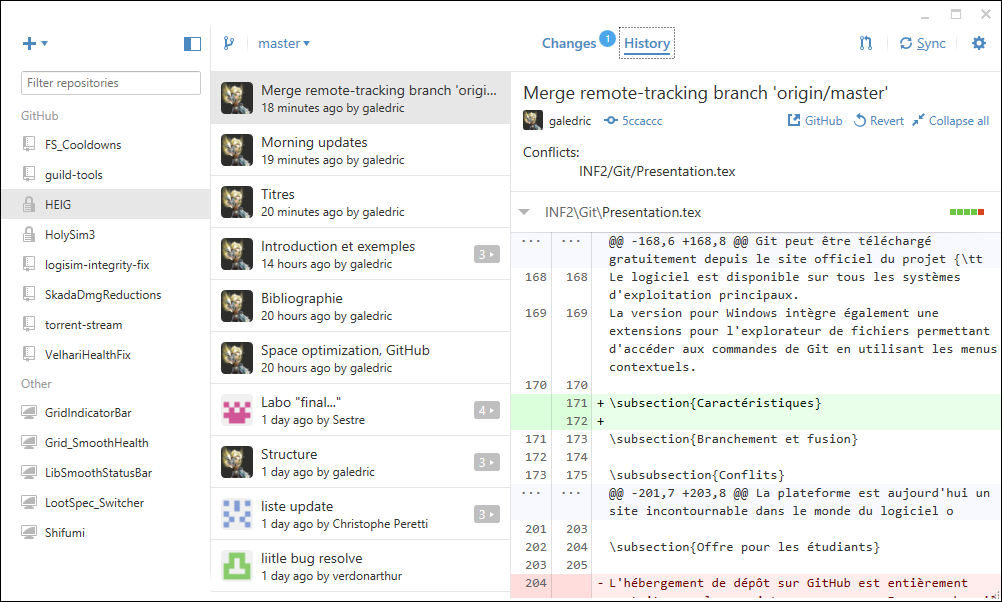
\includegraphics[width=7cm]{img_gh_win}		
			{\tt https://windows.github.com/}
			\vspace{-0.4cm}
		\end{center}
		&
		\begin{center}
			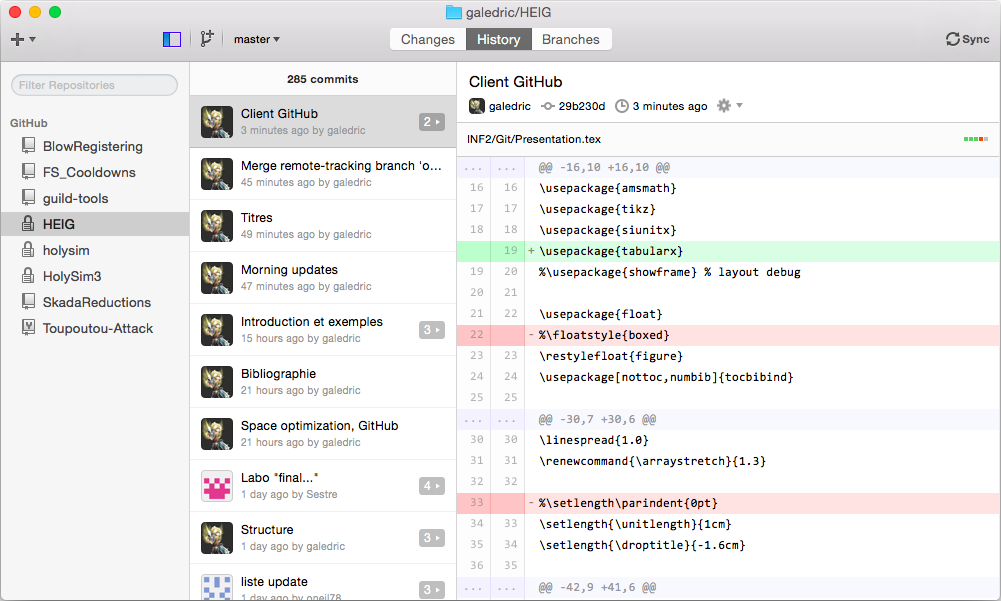
\includegraphics[width=7cm]{img_gh_mac}
			{\tt https://mac.github.com/}
			\vspace{-0.4cm}
		\end{center}
	\end{tabularx}
	\caption{Interface du client GitHub sur Windows et Mac OS}
\end{figure}
\fi %%%

%Il peut être téléchargé aux adresses 
%\begin{enumerate}
%	\item {\tt https://windows.github.com/}
%	\item {\tt https://mac.github.com/}
%\end{enumerate}

Bien qu'il remplisse très bien son rôle dans la plupart des cas, certaines erreurs ou situations très particulières peuvent nécessiter l'utilisation de commande dans le terminal pour rétablir le bon fonctionnement.
Quelques connaissances de Git restent très utiles.

\pagebreak
\begin{thebibliography}{1}

\bibitem{progit}
	CHACON, Scott et STRAUB, Ben. {\em Pro Git} (2e éd). Apress. 2014. \\
	Disponible en ligne: {\tt http://git-scm.com/book/en/v2}

\bibitem{about}
	{\em About Git}. Site du projet Git ({\tt http://git-scm.com/about}). \\
	Consulté le 3 juin 2015.

\bibitem{wiki-git}
	{\em Git}. Wikipedia ({\tt http://en.wikipedia.org/wiki/Git}). \\
	Consulté le 3 juin 2015.

\bibitem{wiki-bk}
	{\em BitKeeper}. Wikipedia ({\tt http://en.wikipedia.org/wiki/BitKeeper}). \\
	Consulté le 3 juin 2015.

\bibitem{wiki-gh}
	{\em GitHub}. Wikipedia ({\tt http://en.wikipedia.org/wiki/GitHub}). \\
	Consulté le 3 juin 2015.
	
\end{thebibliography}

\end{document}